\documentclass[conference]{IEEEtran}
\IEEEoverridecommandlockouts
% The preceding line is only needed to identify funding in the first footnote. If that is unneeded, please comment it out.
\usepackage{cite}
\usepackage{amsmath,amssymb,amsfonts}
\usepackage{mathtools}
\DeclarePairedDelimiter\ceil{\lceil}{\rceil}
\DeclarePairedDelimiter\abs{\lvert}{\rvert}
\usepackage{algorithmic}
\usepackage{graphicx}
\usepackage{textcomp}
%\usepackage{xcolor}
\usepackage[brazilian]{babel}
\usepackage[utf8]{inputenc}
\usepackage[T1]{fontenc}
\def\BibTeX{{\rm B\kern-.05em{\sc i\kern-.025em b}\kern-.08em
    T\kern-.1667em\lower.7ex\hbox{E}\kern-.125emX}}
\usepackage[table,xcdraw]{xcolor} % colored column lines

\graphicspath{{img/}}
\begin{document}

\title{Bancos de Dados de Grafos Distribuídos\\
%{\footnotesize \textsuperscript{*}Note: Sub-titles are not captured in Xplore and
%should not be used}
%\thanks{Identify applicable funding agency here. If none, delete this.}
}

\author{\IEEEauthorblockN{Gustavo Estrela de Matos}
\IEEEauthorblockA{\textit{Instituto de Matemática e Estatísticas} \\
\textit{Universidade de São Paulo}\\
São Paulo, Brasil \\
gestrela@ime.usp.br}
\and
\IEEEauthorblockN{Hector Montenegro Terceros}
\IEEEauthorblockA{\textit{Instituto de Matemática e Estatísticas} \\
\textit{Universidade de São Paulo}\\
São Paulo, Brasil \\
hector@ime.usp.br}
}

\maketitle

\begin{abstract}
    V{\color{blue}amos fazer este por último...}
\end{abstract}

\begin{IEEEkeywords}
component, formatting, style, styling, insert
    {\color{red} Isso aqui eu não entendi direito, não sei como fazer aqui.}
\end{IEEEkeywords}

\section{Introdução}
% Acho que podemos começar falando de grafos e como eles conseguem
% representar diversos objetos da vida real.
%
% No contexto de bancos de dados, os arcos do grafos podem representar
% relacionamentos entre entidades.

% Esse tipo de representação nos permite extrair
% informações complexas sobre relacionamentos de maneira simples, o que
% muitas vezes não é possível em um BD relacional.

% Dar um exemplo disso

% Entretanto, esse tipo de banco de dados pode encontrar alguns desafios...
% Muitas aplicações destes BDs incluem redes tão grandes que não é
% viável o armazenamento em uma única máquina, como exemplo, redes
% sociais. Portanto, é desejável que existam bancos de dados em grafos
% que tem dados distribuídos.

% Além de ter dados distribuídos, é necessário também criar ferramentas
% capazes de conduzir processamentos que permitam extrair informações
% sobre esses grafos, de maneira eficiente e escalável.

% Durante o artigo, vamos apresentar as soluções mais conhecidas para
% enfrentar esses desafios, e também quais as características dos
% principais bancos de dados de grafos, de acordo com os aspectos que
% apresentamos anteriormente.
Grafos são objetos matemáticos que podem ser usados como estruturas de
dados em diversas aplicações computacionais. Sistemas de Bancos de Dados
baseados em grafos são considerados bancos de dados
NoSQL~\cite{nosqlorg} e podem ser aplicados em diversos contextos, como
o de aplicativos da web; áreas industriais de transportes,
telecomunicação e comércio~\cite{neo4jcustomers}; e também em áreas de
pesquisa, como em bioquímica~\cite{biochem4j}, biologia
molecular~\cite{biomol} e web semântica~\cite{sematicweb}.

Um grafo pode ser definido como uma dupla $G = (V, E)$,
em que $V$ é um conjunto de vértices (ou nós) e $E$ é um conjunto de
arcos, que conectam dois nós. Podemos representar um arco $e \in E$,
por uma dupla $e = (v_i, v_j)$ com $v_i \in V$ e $v_j \in V$. No
contexto de bancos de dados de grafos, usualmente um nó representa
uma entidade modelada, e arcos representam relacionamentos entre essas
entidades. É comum que os nós recebam rótulos que estão associados ao
tipo de entidade modelada, e também um conjunto de propriedades em
formato chave-valor, capaz de armazenar atributos da entidade. Além
disso, os arcos do modelo também podem receber rótulos que identificam
o tipo de relacionamento que é modelado, e um conjunto de propriedades
que representam atributos do relacionamento.

Bancos de dados baseados em grafos costumam ser aplicados em contextos
em que os dados de interesse possuem relacionamentos complexos ou
simplesmente quando boa parte da informação está contida nos
relacionamentos. Nestes casos, um banco de dados relacional pode ser
inadequado ou ineficiente. Considere, por exemplo, a relação
{\ttfamily FABRICA (id\_fabricante, id\_produto)}. Em uma consulta em
que se deseja saber as informações dos produtos fabricados por uma
fábrica, no modelo relacional, é necessário fazer uma junção com a
relação que armazena os dados dos produtos, enquanto no modelo baseado
em grafos, basta percorrer os arcos do relacionamento
{\ttfamily FABRICA} que estão ligados ao nó que representa a fábrica de
interesse. Além de ser mais eficiente para algumas consultas, sistemas
baseados em grafos podem ter consultas mais expressivas, capazes de
representar relacionamentos complexos entre os dados~\cite{neo4jquery}.

Assim como outros bancos de dados NoSQL, os bancos de dados em grafos
são muito utilizados em aplicações que precisam armazenar um grande
volume de dados. Para atender a este requisito, alguns bancos de dados
baseados em grafos permitem armazenamento distribuído. Este tipo de
solução precisa implementar particionamento de dados. Além disso, um
sistema distribuído deve providenciar maneiras de responder a consultas
que acessam informações de vértices alocados em diferentes máquinas de
uma rede.

Neste artigo, nosso principal objetivo é apresentar os conceitos
fundamentais e as principais soluções para implementar bancos de dados
baseados em grafos distribuídos, e também sistemas para o processamento
distribuído de grafos. Ao longo deste trabalho, vamos... {\color{blue}
informações a serem adicionadas no futuro, com o que vamos colocar de
fato no artigo}.

\section{Metodologia}
- Como escolhemos os artigos que lemos para criar esse artigo?
- Qual tipo de grafos estamos focados em tratar? (Os que a gente achou...
acho que é maioria usado pra rede social(?))

\section{Conceitos Fundamentais}
Nesta seção apresentamos os conceitos fundamentais para entender o
funcionamento de bancos de dados e ferramentas de processamento de dados
baseados em grafos, mais especificamente, em contextos distribuídos.

\subsection{Graph DBMS versus Graph Analytics Systems}
Para obter os benefícios de um modelo de dados baseado em grafos, é de interesse usar de ferramentas que melhor aproximam esse comportamento. Detalhes adicionais como propriedades, \emph{labels}, direção dos arcos e significados semânticos podem ser usados em modelos mais específicos, como RDF, hipergrafos ou grafos com propriedades. Existem duas categorias de Bancos de Dados de Grafos que são de grande interesse e uso atualmente: \emph{Graph DBMS} e \emph{Graph Analytics Systems}.

\subsubsection{Graph DBMS}
Sistemas de Bancos de Dados de Grafos enfatizam armazenamento persistente e garantias transacionais em um ambiente multi-usuário. A independência lógica e física entre os dados é conquistada pela adoção de um modelo de alto nível do grafo, por exemplo um grafo com propriedades, aliado a uma separação do armazenamento físico. Esses modelos podem ser classificados como nativos (ou seja, com armazenamento específico de grafo) ou não-nativo (usando de outra forma de armazenamento, por exemplo documentos). Exemplos incluem Neo4j, OrientDB, ArangoDB, Gaffer,
SAP Hana Graph, e JanusGraph.

\emph{Graph Analytics Systems} ou \emph{Graph Processing Frameworks} focam-se principalmente em tarefas analíticas sobre grandes grafos, com tolerância a falhas e processamento distribuído. Essas tarefas podem demorar horas e ser realizadas sobre um largo \emph{cluster}, como por exemplo um algoritmo de \emph{PageRank} ou centralidade. São adotados processamentos assíncronos e distribuídos, e se busca reduzir o I/O do cluster. Exemplos desse tipo de ferramenta incluem Pregel, Blogel, Apache Giraph e Gradoop.

A principal diferença entre essas duas classes de ferramentas é no tipo de transação a que dão mais importância e, por outro lado, onde perdas são mais aceitáveis. GDBMS focam-se na garantia de transações de \emph{update}, afetando tipicamente apenas uma porção pequena do grafo, e pagam o custo em tempo e eficiência para essa garantia. GAS, por outro lado, focam-se em tarefas de processamento do grafo inteiro, tipicamente em ambientes distribuídos, adotando perdas de qualidade próximas a outras ferramentas NoSQL.

%\subsection{Notação e representação de grafos (?)}
% vértice adjacente
% caminho mínimo
% diâmetro de um grafo

\subsection{Cortes de grafos}
O conceito de corte em grafo é importante para formalização e análise
do particionamento de um grafo em um contexto distribuído. Para se
trabalhar com grafos de maneira distribuída, é necessário criar um
particionamento do grafo, para que cada parte seja alocada em um nó da
rede de computadores usada. Um particionamento precisa ser feito de
maneira que o processamento do grafo seja balanceado, ou seja, as
máquinas devem ter números de acessos similares; além disso, é
importante fazer com que os processamentos do grafo sejam feitos com o
menor número de nós de computação possível, pois o processamento que
envolve mais de um nó de computação necessita de maior comunicação pela
rede, aumentando a latência da operação. Para analisar estes dois
aspectos com maior formalismo, definimos o conceito de corte.

Um corte é um particionamento em dois conjuntos disjuntos de vértices de
um grafo. Seja $G = (V, E)$ um grafo, então um conjunto $S \subseteq V$
de vértices induz o corte $(S, V \setminus S)$. Um arco $e \in E$ é
chamada de arco do corte se ele atravessa as partes, ou seja, se
$e = (u, v)$ com $u \in S$ e $v \notin S$, ou $u \notin S$ e $v \in S$.
Chamamos de tamanho do corte o número de arcos que são arcos do corte. A
figura~\ref{fig:example_cut} apresenta um exemplo de corte em um grafo.

\begin{figure}
    \begin{center}
        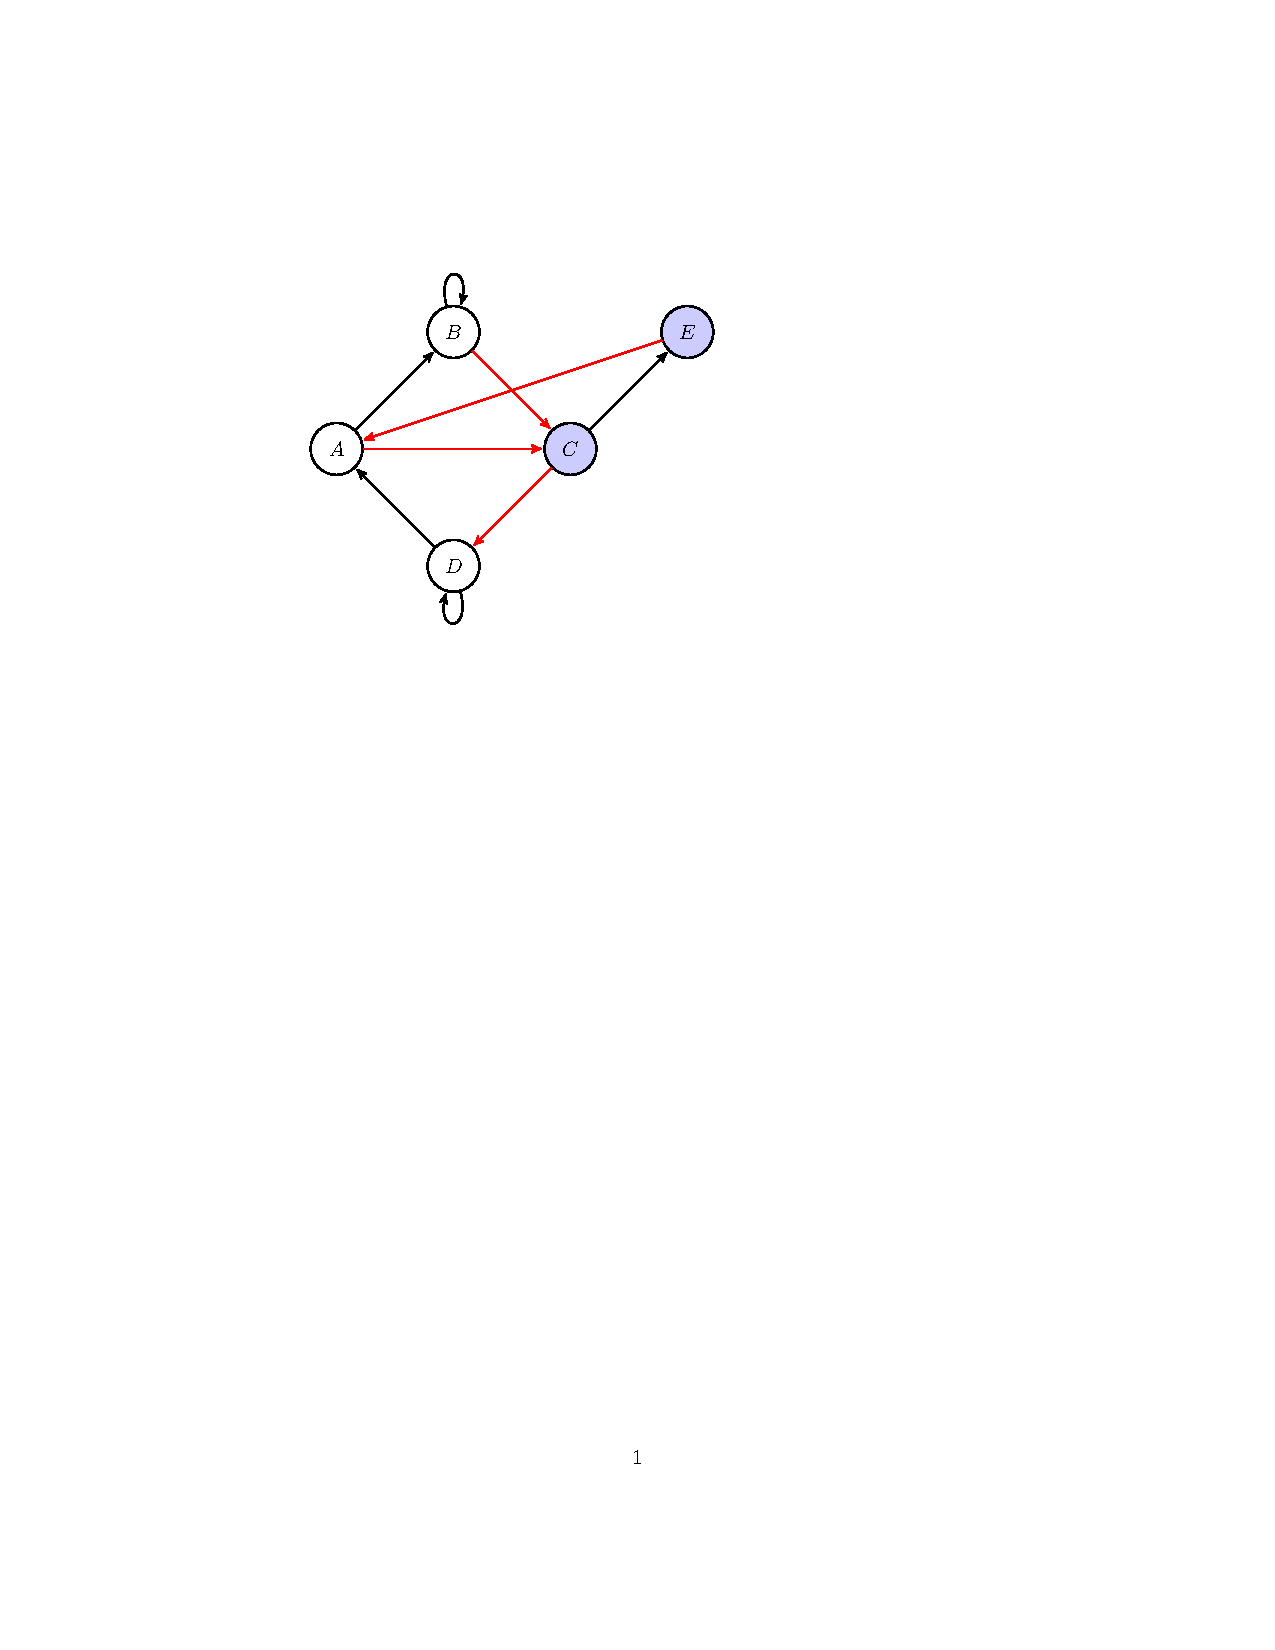
\includegraphics[width=.5\textwidth]{fund_conc/cut_example.pdf}
    \end{center}
    \caption{Grafo com exemplo de corte. O corte apresentado é definido
    pelos conjuntos de vertices ${E, C}$, em azul, e $A, B, D$, em
    branco. Os arcos de cor vermelha são os arcos deste corte. No total,
    são 4 arcos vermelhos neste corte, ou seja, o tamanho deste corte
    é 4.}
    \label{fig:example_cut}
\end{figure}

Note que qualquer particionamento (não apenas bipartições) do conjunto
de vértices de um grafo pode ser realizado após recursivas aplicações de
cortes. Portanto, é possível construir e analisar cortes olhando apenas
para bipartições do grafo original. Perceba também que ao fazer um
particionamento, podemos analisar o balanceamento de processamento
dos nós de computação de acordo com o número de partes (e vértices)
que são alocadas aos nós de computação. Além disso, é possível analisar
a quantidade de comunicação entre nós de acordo com a quantidade de
arcos que conectam diferentes partes, que podem estar alocadas em dois
nós de computação diferentes.

{\color{blue} Se formos falar de cortes baseados em arcos, é melhor
adicionar mais um pedaço de texto explicando esse tipo de corte.}

\section{Particionamento de grafos}
% por que é importante?
% o que podemos analisar do grafo quando fazemos um particionamento
% - balanceamento
% - quantidade de links entre nós
% - e se quisermos levar em conta os nós que são mais acessados?
%   - pomos atualizar estas medidas com  pesos em arcos e nós.
% Quais são as principais abordagens para se fazer um particionamento?
% particionamento online?
O particionamento de um grafo é o processo que permite dividir um grafo
em diferentes partes, que podem ser alocadas em diferentes máquinas,
permitindo o processamento e armazenamento distribuído do grafo. Nesta
seção, apresentaremos três diferentes abordagens de particionamento.
A primeira, baseada no algoritmo METIS~\cite{metis}, é uma heurística
que tenta minimizar a quantidade de arcos que conectam partes
diferentes; a segunda faz um particionamento aleatório; e a terceira
particiona os vértices de acordo com o valor de alguns atributos destes
vértices.

\subsection{Particionamento com cortes mínimos}
O algoritmo METIS tem como objetivo produzir um particionamento com
$k$ partes que minimiza a quantidade de arcos atravessando partes, ou
seja, produz cortes minímos no grafo. O problema de encontrar tal
partição é chamado $k-$particionamento de um grafo, e vamos defini-lo
assim: dado um grafo $G = (V, E)$, com $|V| = n$, particione $V$ em $k$
conjuntos $V_1, V_2, \ldots, V_k$ de maneira que
$V_i \cap V_j = \emptyset$ para $i \neq j$, $\bigcup_{i = 1}^k V_i = V$,
e $|V_i| = n / k$ para $i \in \{1, \ldots, k\}$ (sem perda de
generalidade, se $n$ não é divisível por $k$, então adicione nós
"fantasmas" até que $k | n$). O $k-$particionamento também pode ser
generalizado ao considerar pesos para arcos, adicionando uma informação
de importância ou relevância para as conexões, mas por facilidade vamos
considerar apenas o caso em que todos os pesos dos arcos são iguais, o
que é consistente com a definição que apresentamos. Lembre também que
um corte em um grafo também é uma bipartição do grafo; a escolha por um
dos nomes ao longo desta seção será feita de maneira conveniente à
explicação dos conceitos.

O $k-$particionamento possui importância em aplicações de computação
paralela e distribuída, e foi provado ser
NP-completo~\cite{graphpartitioning}, ou seja, o problema se torna
intratável rapidamente com o aumento da instância. Por isso, o algoritmo
METIS é uma heurística, ou seja, a solução produzida não é ótima em
geral.

A heurística METIS resolve o problema do $k-$particionamento realizando
aplicações recursivas de um procedimento de biparticionamento. O número
total de chamadas recursivas feitas é no máximo $\ceil{\log x}$. O
algoritmo de bipartição é também uma heurística que tenta achar o
corte de menor custo no grafo. Como achar esta partição no grafo pode
tomar muito tempo, uma etapa de encolhimento é feita antes, e depois
disso o grafo bipartido é expandido e refinado até se obter uma
bipartição do grafo original. O algoritmo de biparticionamento é
composto por três etapas:
\begin{itemize}
\item{encolhimento:} pares de vértices são escolhidos dois
    a dois, e são acoplados em um vértice novo que reune todos os arcos
    que estavam nos vértices antigos. Esta etapa é repetida até o
    grafo ser considerado pequeno;
\item{biparticionamento:} uma heurística (novamente) determina um corte
    com tamanho pequeno;
\item{expansão:} os vértices acoplados são desfeitos ao mesmo tempo que
    a bipartição é atualizada de acordo com os novos nós.
\end{itemize}

Durante o encolhimento, os vértices devem ser escolhidos dois a dois sem
repetições, o que é equivalente a escolher um emparelhamento do grafo.
Um emparelhamento é um conjunto de arcos de um grafo que não tem
vértices em comum. O algoritmo METIS implementa uma heurística
de emparelhamento máximo (com maior número de arcos), para escolher os
pares de vértices para serem acoplados. A vantagem de fazer um
emparelhamento máximo durante o encolhimento é diminuir o número de
iterações até que o grafo fique pequeno. Segundo Karypis et al., um
grafo de tamanho 100 é pequeno o suficiente para seguir para etapa de
bipartição.
% TODO: talvez adicionar uma figura de matching aqui

Com o grafo encolhido, uma bipartição deve ser mais facilmente
encontrada. Porém, como este problema ainda é
NP-difícil~\cite{graphpartitioning}, uma outra heurística é usada. Esta
heurística constrói um corte do grafo, e é um algoritmo guloso que
começa com um corte que contém apenas um vértice, escolhido
aleatóriamente, e a cada iteração aumenta o conjunto de vértices do
corte ao adicionar um novo vértice, até que o corte tenha metade dos
vértices do grafo. Em cada etapa do algoritmo, um vértice de fora do
corte que está conectado a um arco do corte é escolhido. Esta escolha é
feita de acordo com o ganho de arcos de corte que o novo vértice pode
adicionar (ou remover) no corte atual. Seja $S_i$ o conjunto de vértices
do corte da $i-$ésima iteração, então, definimos o ganho de adicionar um
vértice como:

\begin{equation}
    g_v = \abs{\{u \mid (v, u) \in E, u \notin S_i\}} -
          \abs{\{u \mid (v, u) \in E, u \in S_i\}}
\end{equation}

A medida $g_v$ também é útil para a última etapa do biparticionamento,
que ao mesmo tempo que expande o grafo colapsado, faz um refinamento do
biparticionamento produzido. A cada iteração desta etapa, um nó é
desacoplado e então todos os vértices da borda do corte do
biparticionamento são analisados para uma possível troca de partes. Na
prática, esta etapa é aplicada com otimizações que tornam desnecessário
analisar todos os vértices da borda por várias iterações, tornando essa
heurística mais eficiente.

O algoritmo METIS é até hoje um dos principais algoritmos de
particionamento de grafos, e por isso é usado como base de comparação
para outras propostas~\cite{baselinemetis}.


\subsection{Particionamentos aleatórios e por intervalos}
Um particionamento aleatório atribui partes aos vértices de maneira
aleatória e uniforme. Esta atribuição é feita de acordo com alguma
função de hash, que pode ser aplicada, por exemplo, no atributo
de identificação do vértice. Este tipo de particionamento é facilmente
implementado visto que o único requisito é que uma função de hash
distribua os vértices de maneira equilibrada entre os nós.

Um particionamento por intervalo é similar, e também precisa de uma
função de hash, mas ao invés de atribuir partes a valores de um
atributo, essa função atribui partes a intervalos dos valores de
atributos. Esta abordagem é útil quando há um atributo nos vértices que
determina a chance de relacionamento entre vértices de acordo com
seus valores; por exemplo, se os vértices são pessoas com um atributo
de latitude e longitude, então é razoável adimitir que os
relacionamentos (arcos) ocorrerão mais entre pessoas que tem valores
próximos para esses atributos.

Além de ser facilmente implementadais, essas estratégias precisam de
pouco processamento e pouco espaço de memória para identificar a qual
parte um vértice foi alocado. Outra vantagem desses métodos é que um
novo vértice do grafo pode ser atribuido para uma parte de maneira
rápida, diferente da abordagem de cortes mínimos.

\subsection{Comparação entre abordagens de particionamento}
Ambas abordagens apresentadas anteriormete podem ser aplicadas
vantajosamente. A estratégia baseada em cortes se aproveita da estrutura
da estrutura do problema de interesse e pode produzir um particionamento
que possui poucos arcos conectando duas partes, ou seja, um
particionamento que agrupa as entidades que se relacionam constantemente
e, portanto, faz as consultas precisarem de menos comunicações entre
nós de computação. No caso dos particionamentos aleatórios ou por
intervalos, o processo de particionamento é simples de se implementar
e necessita de pouco espaço de armazenamento. Além disso,
particionamentos aleatórios podem atribuir partes a novos vértices assim
que eles são criados.

Por outro lado, ambas abordagens também possuem desvantagens. A
principal desvantagem do particionamento por cortes é a sua
complexidade, de implementação e de recuperação das partes. Além disso,
no particionamento baseado em cortes, uma política precisa ser definida
para quando um novo vértice é criado: este vértice precisa ser
eventualmente colocado em alguma parte, mas deve ser considerado que
refazer todo processo de particionamento sempre que um novo nó é criado
é inviável. A desvantagem do método particionamento aleatório e não
usar a estrutura dos dados do problema, o que pode fazer com que
operações comuns causem um grande tráfego na rede, pois os nós
fortemente relacionados não estarão disponíveis nos mesmos locais.

O trabalho de Khayyat et al. mostra que, de fato, não um consenso de
qual é a melhor alternativa de particionamento~\cite{mizan}. Portanto,
a escolha de uma estratégia de particionamento depende da aplicação. A
tabela~\ref{tab:partitions} apresenta os principais aspectos
estratégias de particionamento que apresentamos nesta seção.

\begin{table}[]
\centering
\caption{Características de abordagens de particionamento}
\label{tab:partitions}
\begin{tabular}{lcc}
\hline
& \begin{tabular}[c]{@{}c@{}}Particionamento \\
    de corte mínimo
  \end{tabular} &
  \multicolumn{1}{c}{\begin{tabular}
            [c]{@{}c@{}}Particionamento aleatório \\
             e por intervalo
  \end{tabular}} \\ \hline

\\
Usa estrutura do grafo & Sim & Não \\
\\
\rowcolor[HTML]{DFDFDF}
\begin{tabular}[c]{@{}l@{}}Dificuldade de cálculo \\
    do particionamento
\end{tabular}  & Difícil & Fácil \\
\\
\begin{tabular}[c]{@{}l@{}}Necessita de armazenar\\
        partes explicitamente
\end{tabular} & Sim & Não \\
\\
\rowcolor[HTML]{DFDFDF}
    \begin{tabular}[c]{@{}l@{}}Atribuição de parte para\\
        um novo vértice
    \end{tabular} & \begin{tabular}[c]{@{}c@{}}Depende de criação \\
        de política
    \end{tabular}  & Automática
\\
\end{tabular}
\vspace{1em}
\end{table}

\section{Sistemas Gerenciadores de Bancos de Dados em Grafos}

Os Sistemas Gerenciadores de Bancos de Dados em Grafos, a seguir referenciados como SGBDG, são as ferramentas que focam-se em manter todas as garantias de um SGBDR, mas usando de uma representação de dados voltada a Grafos ao invés de Relações. Portanto, essas ferramentas são focadas em tarefas OLTP, com acesso de baixa latência a pequenas partes do grafo, e trazem vantagens como garantia de persistência e otimização de \emph{queries} \cite{nole-sartiani}. Muitos sistemas desse tipo são centralizados, como por exemplo Neo4j~\cite{neo4j} e OrientDB~\cite{orientdb}, que entretanto oferecem replicação como uma solução para fornecer alta disponibilidade para consultas de leitura, mas já estamos vendo o surgimento e popularização de sistemas distribuídos, como JanusGraph~\cite{janusgraph}, Horton+ \cite{horton} e ThingSpan~\cite{thingspan}. Esses últimos são tipicamente construídos sobre um \emph{backend} distribuído, como Apache Hadoop ou Cassandra, visando a construção de um sistema em que os servidores do \emph{cluster} não compartilham nenhum recurso, e o sistema então se ocupa da tarefa de comunicação interna.

Todas essas ferramentas implementam alguma forma de consulta aos dados. Várias possuem sua própria linguagem de consulta declarativa, como a Cypher do Neo4j, uma linguagem de checagem sobre todo o grafo, como a Gremlin da Apache TinkerPop usada no JanusGraph e OrientDB, ou mesmo uma extensão da SQL que permita a expressão de transversais no grafo, como está disponível no OrientDB. Também é muito comum que sejam disponibilizadas APIs para processamento de transações e processamento de tarefas. A maioria dessas linguagens não possui interpretação semântica nativa, a exceção sendo SPARQL, uma linguagem montada para a consulta de bancos de dados de RDF, que por vezes é disponibilizada nas ferramentas aqui apresentadas.

Um tipo de ferramenta que possui muitas características similares a SGBDG, incluindo conexões diretas entre itens de dados e uma linguagem própria de consulta, são os bancos de dados de RDF (\emph{Resource Description Framework}), com a linguagem SPARQL. Cada item de RDF é uma relação entre duas entidades também presentes no BD, então a tradução dessa relação como um arco entre nós representantes das entidades é natural, o que aproxima tais tipos de ferramentas. Inclusive, muitas ferramentas de SGBDG permitem que um usuário traduza uma consulta SPARQL em uma na linguagem própria da ferramenta, potencializando o conhecimento acumulado em SPARQL e a expressividade semântica dessa linguagem. Entretanto, essas ferramentas estão fora do escopo do presente trabalho.

\subsection{Neo4j}

Neo4j~\cite{neo4j} é o SGBDG mais popular atualmente, de acordo com o ranking DB-Engines \cite{db_engines}. É um SGBDG nativo, centralizado, com uma versão \emph{open-source} (\emph{Community}) e uma restrita (\emph{Enterprise}). Na versão \emph{open-source}, são disponíveis a linguagem de consulta Cypher e APIs para várias linguagens de programação (.Net, Java, JavaScript, Go, e Python), além das garantias de transação similares a ACID. Na versão paga, há extensões como a implementação em um \emph{cluster}, com replicação completa do grafo para agilizar transações de consulta simultâneas, mas sem \emph{sharding} ou particionamento do grafo original. Também são oferecidas nessa versão ferramentas de \emph{backup online} e gerenciamento de acessos. Uma visão geral dessa ferramenta está na figura \ref{fig:neo4j}. O Neo4j usa do \emph{Property Graph Model}, um grafo direcionado e onde se representam os nós, arcos e propriedades de nós ou arcos, que são guardadas em três arquivos separados

\begin{figure}[htbp]
\centerline{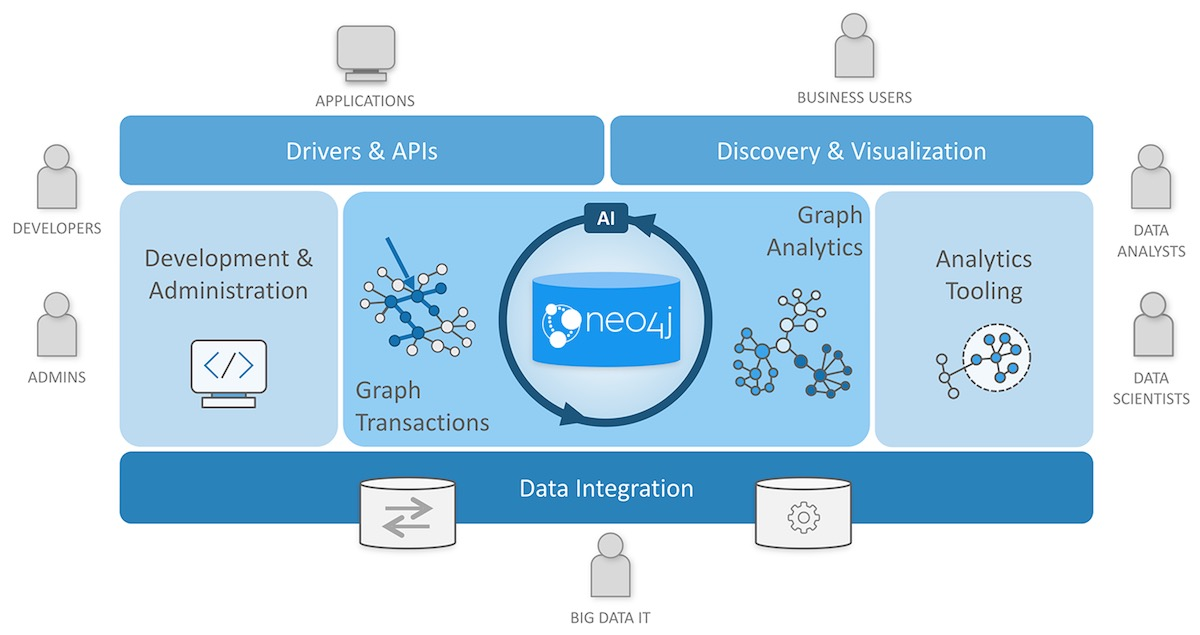
\includegraphics[width=0.9\linewidth]{img/neo4j/neo4j_graph_platform.jpg}}
\caption{Ilustração das capacidades do Neo4j, especialmente sua integração com vários tipos de usuários e suas ferramentas.}\label{fig:neo4j}
\label{fig}
\end{figure}

A linguagem Cypher é declarativa, inspirada no SQL e estendida visando a expressão de estruturas do grafo a serem procuradas. Essa linguagem se baseia numa sintaxe com as cláusulas \emph{START-SELECT-WHERE-RETURN}. \emph{START}, opcional, declara um nó específico de onde iniciar a transversal. \emph{SELECT} define o padrão a ser buscado, tipicamente em nós e as relações entre eles. \emph{WHERE} permite a filtragem a partir de propriedades e outras comparações. \emph{RETURN} aponta que informações devem ser retornadas, inclusive permitindo funções de agregação.

Rudimentos de \emph{ASCII-art} são usados na expressão de padrões a ser buscados pela cláusula \emph{SELECT}, com nós do grafo representados por parênteses $()$ e arcos representados por dois traços $--$, possivelmente com uma direção especificada $-->$ ou $<--$. Essas estruturas podem ser melhor especificadas usando de tipos e \emph{labels} para relações e nós respectivamente, e de propriedades dessas entidades. O otimizador de query sabe usar dessas especificações para limitar o escopo das transversais sobre o grafo, agilizando as consultas apropriadamente. Cada entidade da expressão pode receber uma variável local, que é então usada nas cláusulas \emph{WHERE} e \emph{RETURN} para o tratamento dos dados retornados.

No exemplo da figura \ref{fig:neo4j2}, a query busca um nó de label Pessoa, com uma propriedade "name" tendo valor "Jennifer", que tenha uma relação de tipo WORKS\_FOR com um nó de label "Company". Desse último nó, ela retorna a propriedade "name".

\begin{figure}[htbp]
\centerline{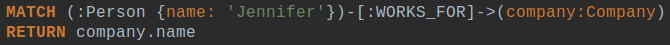
\includegraphics[width=0.9\linewidth]{img/neo4j/neo4j_ps2.png}}
\caption{Exemplo de query em Cypher}\label{fig:neo4j2}
\label{fig}
\end{figure}

\subsection{OrientDB}

OrientDB~\cite{orientdb} é um SGBD que suporta modelos de documentos, grafos, chave-valor e objetos, com o principal atrativo sendo a capacidade de trabalhar mais de um desses formatos no mesmo gerenciador, criando uma base de dados multi-modelo. Os dados são armazenados como documentos de chave-valor, em que cada valor pode ser um dado primitivo, documentos internos ou listas de outros documentos, e são agrupados em "classes". De nosso principal interesse é a forma como o SGBDG implementa \emph{links} entre esses documentos, que são processados sempre que um documento é processado, de forma a agilizar as transversais que são de interesse em grafos.

Usado como grafo, cada nó do grafo é armazenado como um registro com um ID próprio e as listas de arcos incidentes (entrando ou saindo), e cada arco também é armazenado com um ID próprio, seus nós de saída e chegada (chamados cabeça e cauda), e um \emph{label} para o tipo de relacionamento entre os vértices. Ambas as entidades, como documentos sem esquema restrito, podem receber qualquer quantidade de propriedades a mais como campos chave-valor. Como todo registro no SGBD possui um ID próprio, o acesso a tais registros é rápido e direto, evitando o processamento de longas listas.

Evitando criar uma nova linguagem de consulta, OrientDB implementa o SQL estendido para funcionalidades de grafos, mantendo a sintaxe \emph{SELECT-FROM-WHERE-GROUP BY} e encapsulamento de consultas, mas perdendo a cláusula \emph{HAVING}. A navegação pelas relações entre os registros do BD é feita através dos links presentes nos registros, e referenciada por \emph{dot notation}. Por exemplo, assumindo que registros da classe \emph{Employee} possuam uma propriedade \emph{city} com um link para registros dessa classe, realizar uma consulta para extrair apenas empregados de uma dada cidade é fácil como mostrado na figura \ref{fig:orientdb_ps1}. Também é possível aplicar funções sobre valores retornados (por exemplo, \emph{sum} para uma agregação), ou usar de métodos nos próprios pares chave-valor, como na figura \ref{fig:orientdb_ps2}.

\begin{figure}[htbp]
\centerline{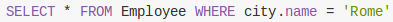
\includegraphics[width=0.9\linewidth]{img/orientdb/orientdb_ps1.png}}
\caption{Empregados na cidade de 'Rome', no OrientDB SQL.}\label{fig:orientdb_ps1}
\label{fig}
\end{figure}

\begin{figure}[htbp]
\centerline{
\includegraphics[width=0.9\linewidth]{img/orientdb/orientdb_ps2.png}}
\caption{Retornando o primeiro e último nome de cada empregado concatenados, no OrientDB SQL.}\label{fig:orientdb_ps2}
\label{fig}
\end{figure}

\subsection{JanusGraph}

JanusGraph~\cite{janusgraph} é um SGBDG não-nativo distribuído e \emph{open-source}, voltado ao processamento de grafos maiores do que as capacidades de uma só máquina. Usando de uma arquitetura modular, permite a implementação de um ou mais \emph{backends} de armazenamento de dados e índices, e comunicação a aplicações e usuários por uma API Gremlin. Ao contrário da maioria dos SGBDGs, JanusGraph é dependente de esquemas, definidos sobre os nós, arcos e propriedades, mas esse esquema pode tanto ser declarado quanto inferido no uso, e alterado conforme o grafo evolui.

A arquitetura modular do \emph{backend} permite o uso de diferentes ferramentas, dependendo dos objetivos da modelagem. Em especial, casos de uso em que a manutenção da consistência da leitura é garantia necessária são bem servidos pela Apache HBase, ao custo de uma chance de requisições falharem. Por outro lado, Apache Cassandra é o \emph{backend} sugerido no caso de preferência de disponibilidade contra a completude do resultado. Essas ferramentas já estão integradas ao ecossistema Apache Hadoop, e existe a possibilidade de construção de adaptadores para outros \emph{backends} de acordo com a necessidade do usuário. Essa arquitetura está graficamente descrita na figura \ref{fig:janusgraph_ps1}.

\begin{figure}[htbp]
\centerline{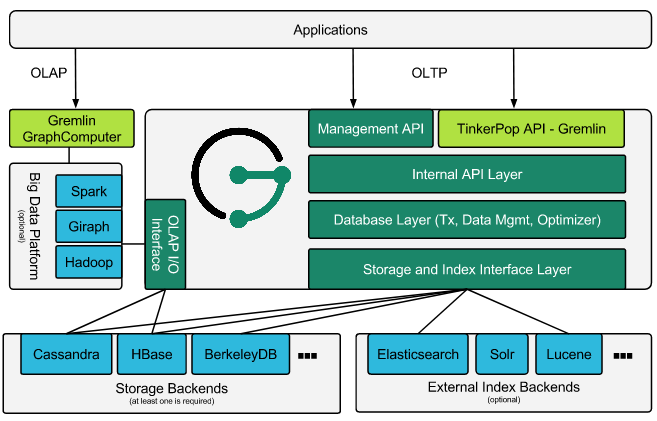
\includegraphics[width=0.9\linewidth]{img/janusgraph/janusgraph_ps1.png}}
\caption{Arquitetura do JanusGraph}\label{fig:janusgraph_ps1}
\label{fig}
\end{figure}


Consultas são realizadas usando da linguagem Gremlin, uma linguagem funcional componente do Apache TinkerPop. Nela, operadores de transversal, representando relações entre nós através de arcos, são encadeadas formando uma expressão representante do caminho a ser buscado. Cada passo dessa expressão retorna objetos, que serão processados pelo próximo passo, de forma que a sintaxe não é restrita como a de outras linguagens apresentadas nesse trabalho. No exemplo da figura \ref{fig:janusgraph_ps2}, foi usado um grafo de exemplo listando a mitologia romana, em que a partir de uma transversal $g$ do grafo, encontra-se o nó referente ao herói \emph{hércules}, encontram-se os vértices de seu pai e avô, e retorna-se afinal o nome desse último, \emph{saturno}.

\begin{figure}[htbp]
\centerline{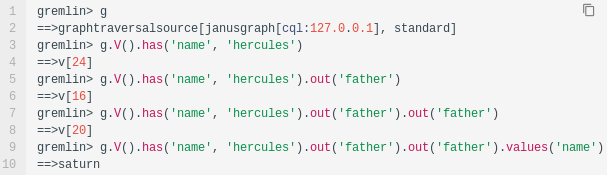
\includegraphics[width=0.9\linewidth]{img/janusgraph/janusgraph_ps2.png}}
\caption{Exemplo de consulta na linguagem Gremlin.}\label{fig:janusgraph_ps2}
\label{fig}
\end{figure}

Uma vantagem de usar a linguagem Gremlin e seu framework, Apache TinkerPop, é que são agnósticos em relação ao SGBDG usado, e aceitos por muitos dos SGBDG, inclusive todos desse trabalho. Para o JanusGraph, isso significa uma forma fácil de integração com outras ferramentas e aplicações, que devem simplesmente interagir com o Gremlin API e construir consultas que esse possa trabalhar.

\subsection{Horton+}
\cite{horton}

\subsection{ThingSpan}
\cite{thingspan}

\section{Graph Analytics Systems}
Com o crescimento das aplicações na internet e em outras áreas como
transportes e comércio, a demanda por processamento eficiente e
distribuído de grafos cresceu. Outros arcabouços de processamento
distribuído com propósitos mais genéricos, como MapReduce, podem não ser
adequados para alguns problemas de grafos. Por isso, tornou-se
necessário a criação de arcabouços de processamento distribuído
especializados em grafos, que permitem escrever programas que fazem
cálculos sobre grafos de maneira mais intuitiva e eficiente. Chamamos
estes arcabouços de {\em Graph Analytics Systems} (GASs).

Uma das primeiras soluções GAS foi o sistema Pregel, criado por
engenheiros do Google~\cite{pregel}. Pregel possui uma abordagem de
processamento centrada nos vértices do grafo. Os programas deste
arcabouço funcionam com uma sequência de rodadas chamadas de {\em
supersteps}; a cada {\em superstep} um vértice pode receber uma
mensagem, fazer uma computação, enviar uma mensagem, ou decidir parar.
Um programa acaba quando todos os vértices decidem parar. Este método de
computação também é a base para outros GAS, como o Giraph~\cite{giraph},
Surfer~\cite{surfer}, GoldenOrb~\cite{goldenorb} e Mizan~\cite{mizan}.
Estas variações do sistema Pregel normalmente se diferenciam pelo
sistema de armazenamento utilizado e também pelo tipo de particionamento
de grafo utilizado.

O sistema Pregel e suas variantes podem ainda não ser adequados para
algumas aplicações, principalmente aquelas em que são construídos grafos
densos. Em um grafo denso, a quantidade de arcos pode ser muito grande,
criando um alto tráfego de informação localmente e também entre os nós
de computação. Como solução para este problema o sistema Blogel foi
desenvolvido. Este sistema utiliza o mesmo método de processamento que o
Pregel, porém faz cálculos centrados em blocos de vértices, evitando
comunicação excessiva entre vértices.

Vamos, nesta seção, explicar em maiores detalhes os funcionamentos dos
arcabouços Pregel e Blogel.

\subsection{Pregel}
% Surfer [4] utilizes min-cut graph partitioning to improve the
% performance of distributed vertex centric graph processing
Pregel é um arcabouço criado por engenheiros do Google, para
processamento de grafos. Este arcabouço surgiu por conta da inadequação
de outros arcabouços de processamento, como MapReduce, no processamento
de grafos. Apesar de surgir como uma alternativa ao MapReduce, Pregel
utiliza uma ideia de sucesso do primeiro arcabouço: processamento
particionado e local. Um programa Pregel é composto por uma sequência
de iterações, chamadas de {\em supersteps} em que cada vértice do grafo
faz processamentos independentes que podem compor a resposta do
programa.

Em cada {\em superstep} um vértice pode receber uma mensagem, fazer um
processamento, ou enviar uma mensagem (ou qualquer combinação dos três).
Um vértice é capaz de receber uma mensagem que lhe foi enviada na
iteração anterior, e esta mensagem normalmente é utilizada como
argumento para algum processamento que o vértice pode ter na iteração. O
processamento de cada vértice é determinado pelo usuário, que escreveu o
programa no arcabouço. Além de receber uma mensagem e fazer um
processamento, um vértice também pode enviar uma mensagem, que será
recebida pelo destinatário na próxima iteração. Um vértice normalmente
envia mensagens para vértices adjacentes, mas uma mensagem também pode
ser enviada para qualquer outro vértice.

\begin{figure}
    \begin{center}
        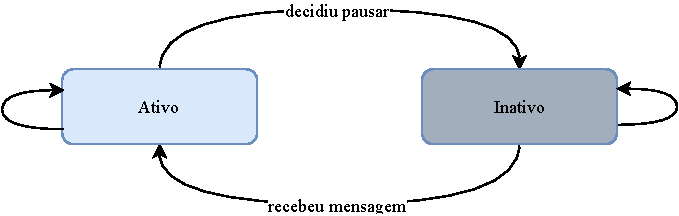
\includegraphics[width=.45\textwidth]{pregel/vertex_state.pdf}
    \end{center}
    \caption{Diagrama de estado de um vértice em um programa Pregel.}
    \label{fig:pregel_states}
\end{figure}

Além fazer trocas de mensagens e processamento, um vértice também pode
pausar. Quando isto acontece, o vértice fica em estado inativo e não faz
nenhum tipo de processamento ou envio de mensagens; por outro lado, um
vértice inativo pode voltar a ser ativo se ele receber uma mensagem. A
figura~\ref{fig:pregel_states} mostra o diagrama de estados de vértices
em um programa Pregel.  Quando todos os vértices estão em estado
inativo, então não existe mais nenhum processamento ou comunicação a ser
feito, logo o programa termina. A figura~\ref{fig:execution_example}
mostra um exemplo de programa em Pregel.

\begin{figure}
    \begin{center}
        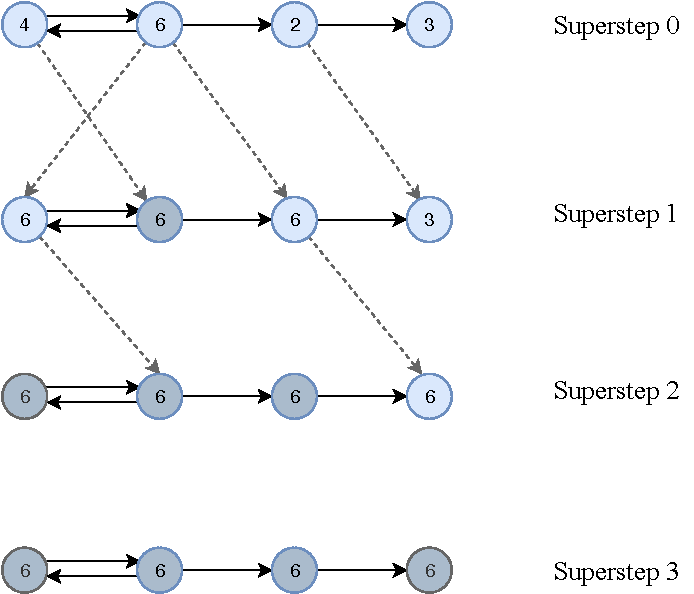
\includegraphics[width=.45\textwidth,
        clip]{pregel/execution_example.pdf}
    \end{center}
    \caption{Exemplo de execução de um programa Pregel, que encontra o
    valor máximo dos vértices de um grafo. Os vértices mais escuros
    estão inativos, enquanto os vértices ativos possuem coloração mais
    clara. Os arcos tracejados representam comunicação entre {\em
    supersteps}, enquanto os arcos sólidos representam os arcos do grafo
    original. Em cada iteração um vértice ativo recebe o valor de um
    vértice adjacente que estava ativo na ultima iteração. Se o valor
    recebido por um vértice é maior do que o seu valor, então este
    vértice propaga o maior valor para todos os seus vértices
    adjacentes; se o valor recebido não for maior que o seu, então o
    vértice decide se tornar inativo.
    }
    \label{fig:execution_example}
\end{figure}

%
% Comentar sobre as outras ferramentas baseadas em Pregel?
%
Após a introdução do sistema Pregel, outros sistemas similares foram
criados. Alguns desses sistemas mudam pontualmente alguns aspectos do
sistema Pregel, incluindo o algoritmo de particionamento utilizado.
O sistema Pregel usa particionamento aleatório, com {\em hashing}, por
padrão~\cite{pregel}, mas outros sistemas similares como Giraph e Surfer
permitem o particionamento por intervalos de valores e cortes mínimos,
respectivamente.

\subsection{Blogel}
% - growing need to deal with massive graphs -> pregel.
% -> pregel e seus clones são alternativas centradas em vértices que
%  trouxeram grandes avanços, porém esses sistemas negligenciam
%  características estruturais de grafos massivos da vida real.
% -> grafos massivos da vida real podem ter a distribuição de arcos
%  concentradas em alguns vértices ou conjuntos de vértices específicos,
%  fazendo com que um programa Pregel tenha um desbalanço de trabalho.
%  Além disso, grafos da vida real podem ter um diâmetro muito grande,
%  ou seja, existem pares de vértices do grafo que estão separados por
%  muitos arcos de distância, o que pode causar um número muito grande
%  de iterações em um algoritmo Pregel.
%  Para solucionar estas dificuldades, o sistema Blogel foi proposto.

% -> Blogel é uma proposta block-centric
% -> simples como Pregel
% -> o que é bloco

% -> como blogel propões resolver o problema

% -> como garantir isso /\? Oras bolas, com o algoritmo de
%  particionamento "correto"

O sistema Pregel surgiu de um contexto em que as aplicações necessitavam
processar grafos massivos, com número muito grande de vértices e
arestas, e este sistema de fato trouxe melhorias nesta área, além de
servir como inspiração para diversos outros sistemas similares. Apesar
disso, a abordagem de processamento centrada em vértices proporciona um
processamento local que negligencia a estrutura global do grafo.

D. Yan et al. consideram que boa parte dos grafos massivos observados em
aplicações reais podem ter seus arcos distribuídos de maneira não
uniforme, concentrados em vértices ou conjuntos de vértices que são
principais no grafo~\cite{blogel}. Este tipo de estrutura faz com que a
divisão de trabalho no Pregel seja desequilibrada entre os nós de
computação. Além disso, outra característica pontuada por D. Yan et al.
é que alguns grafos de interesse podem ter diâmetro muito grande, ou
seja, dois vértices do grafo podem estar separados por muitos arcos de
distância. Neste caso, um algoritmo Pregel pode precisar de um número
muito alto de iterações para que uma mensagem de um vértice alcance seu
destinatário. Para enfrentar estas dificuldades, D. Yan et al.
propuseram um sistema similar ao Pregel, mas que possui um processamento
centrado em blocos de vértices.

O sistema Blogel usa as mesmas ideias de processamento que o sistema
Pregel, porém permite definir uma estrutura de bloco, que assim como os
vértices são capazes de realizar processamentos e trocar mensagens. Um
bloco é simplesmente um conjunto de vértices do grafo. Para que os
problemas apontados por D. Yan et al. sejam enfrentados, é necessário
fazer com que a estrutura de blocos agrupe vértices que se relacionam
constantemente, evitando comunicação excessiva e desnecessária entre
vértices.

Note que escolher um conjunto de blocos para o grafo é novamente fazer
um particionamento do grafo original, e isto pode ser feito de diversas
maneiras. No caso do sistema Blogel, o particionamento escolhido para a
criação dos blocos é implementado utilizando uma abordagem que agrupa
vértices que estão próximos (a menos arcos de distância), mais
especificamente, utilizando um diagrama de Voronoi do grafo. Um diagrama
de Voronoi é uma estrutura que permite decompor um espaço em células
(blocos) que estão centradas por pontos deste espaço. É importante notar
que a noção de distância que é utilizada nesta decomposição não é
baseada em um sistema de coordenadas para os vértices do grafo, o que
pode ser mais comum em outras aplicações desta técnica, mas sim na noção
de menor caminho entre dois vértices.

Experimentos realizados por D. Yan et al. mostraram que, de fato, o
sistema Blogel permite melhor desempenho quando comparado ao Pregel, no
processamento de grafos que possuem uma distribuição não uniforme de
arcos entre os vértices, ou que possuem um diâmetro muito grande.

\begin{thebibliography}{00}
\bibitem{nosqlorg} ``NoSQL Databases'', http://nosql-database.org/.
\bibitem{neo4jcustomers} ``Neo4j Customers'',
    https://neo4j.com/customers/.
\bibitem{neo4jquery} M. Hunger, R. Boyd. ``RDBMS \& Graphs: SQL vs.
    Cypher Query Languages'' Neo4j Blog. Mar. 2016.
        https://neo4j.com/blog/sql-vs-cypher-query-languages/
\bibitem{biochem4j} N. Swainston et al., ``biochem4j: Integrated and
    extensible biochemical knowledge through graph databases'', PLOS
        ONE, vol. 12, no. 7, p. e0179130, Jul. 2017.
\bibitem{biomol} F. Olken, ``Graph Data Management for Molecular
    Biology'', OMICS: A Journal of Integrative Biology, vol. 7, no. 1,
        pp. 75–78, Jan. 2003.
\bibitem{sematicweb} B. McBride, ``Jena: a semantic Web toolkit,” IEEE
    Internet Computing, vol. 6, no. 6, pp. 55–59, Nov. 2002.
\bibitem{metis} Karypis, G., \& Kumar, V. (1998). ``A Fast and High
    Quality Multilevel Scheme for Partitioning Irregular Graphs''. SIAM
        Journal on Scientific Computing, 20(1), 359–392.
        https://doi.org/10.1137/s1064827595287997
\bibitem{graphpartitioning} Andreev, K., \& Racke, H. (2006). ``Balanced
    Graph Partitioning''. Theory of Computing Systems, 39(6), 929–939.
        https://doi.org/10.1007/s00224-006-1350-7
\bibitem{baselinemetis} D. Avdiukhin, S. Pupyrev, e G. Yaroslavtsev,
    ``Multi-dimensional balanced graph partitioning via projected
        gradient descent'', Proceedings of the VLDB Endowment, vol. 12,
        nº 8, p. 906–919, abr. 2019.
\bibitem{mizan} Z. Khayyat, K. Awara, A. Alonazi, H. Jamjoom, D.
    Williams, e P. Kalnis, ``Mizan'', in Proceedings of the 8th ACM
        European Conference on Computer Systems - EuroSys ’13, 2013.
\bibitem{pregel} G. Malewicz et al., ``Pregel'', in Proceedings of the
    2010 international conference on Management of data - SIGMOD ’10,
        2010.
\bibitem{giraph} Avery, Ching. ``Giraph: Large-scale graph processing
    infrastructure on hadoop.'' Proceedings of the Hadoop Summit. Santa
        Clara 11.3 (2011): 5-9.
\bibitem{surfer} Chen, Rishan, et al. ``Improving large graph processing
    on partitioned graphs in the cloud.'' Proceedings of the Third ACM
        Symposium on Cloud Computing. ACM, 2012.
\bibitem{goldenorb} GoldenOrb. A Cloud-based Open Source Project for
    MassiveScale Graph Analysis. http://goldenorbos.org/, 2012
\bibitem{blogel} D. Yan, J. Cheng, Y. Lu, e W. Ng, ``Blogel'',
    Proceedings of the VLDB Endowment, vol. 7, nº 14, p. 1981–1992, out.
        2014.

\bibitem{sahu} Sahu, Siddhartha et al. ``The Ubiquity of Large Graphs and Surprising Challenges of Graph Processing: Extended Survey'' The VLDB Journal (2019): n. pag. Crossref. Web.
\bibitem{nole-sartiani} {\color{red} preciso pegar essa referencia certinha} M. Nolé, C. Sartiani, ``Graph Management Systems: A Survey''
\bibitem{neo4j} ``The Neo4j Getting Started Guide v3.5'',
    https://neo4j.com/docs/getting-started/current/
\bibitem{orientdb} ``OrientDB Manual - version 3.0.14'',
    https://orientdb.org/docs/3.0.x/
\bibitem{tinkerpop} ``Apache TinkerPop'',
    http://tinkerpop.apache.org/
\bibitem{janusgraph} {\color{red} preciso pegar essa referencia certinha}
\bibitem{horton} M. Sarwat, S. Elnikety, Y. He, and M. F. Mokbel, ``Horton+: A Distributed System for Processing Declarative Reachability Queries over Partitioned Graphs'', PVLDB, vol. 6, no. 14, pp. 1918–1929, 2013.
\bibitem{thingspan} ``ThingSpan'' [Online]. Available: http://www.objectivity.com/products/thingspan/.
\end{thebibliography}
\end{document}
